
\chapter{Single-core Design}
\startcontents[chapters]
\printcontents[chapters]{}{1}{}
\noindent\\
While the majority of this report will focus on the multi-processing functionality of this project, it is important understand the design decisions of the single core that will be instantiated many times.

\section{Introduction}
A single-core processor will be instantiated multiple times and each will be connected to a communication bus.

\section{Design and Implementation}
The single-core design is a traditional 5-stage RISC processor (fetch, decode, execute, memory, write-back). The core uses separate instruction and data memories in the style of a Harvard architecture \cite{harvard}.

To satisfy \ref{cd:vendor}, the Verilog code will be self-contained in a single file. This reduces the hierarchical complexity and eases cross-vendor project set-up as only a single file is required to be included. 
A disadvantage with this single file approach is that some external Verilog verification tools that I plan to use, such as Verilator, do not currently support multiple Verilog modules (due to an unfixed bug) within a single file. 

\begin{figure}[H]
\centering 
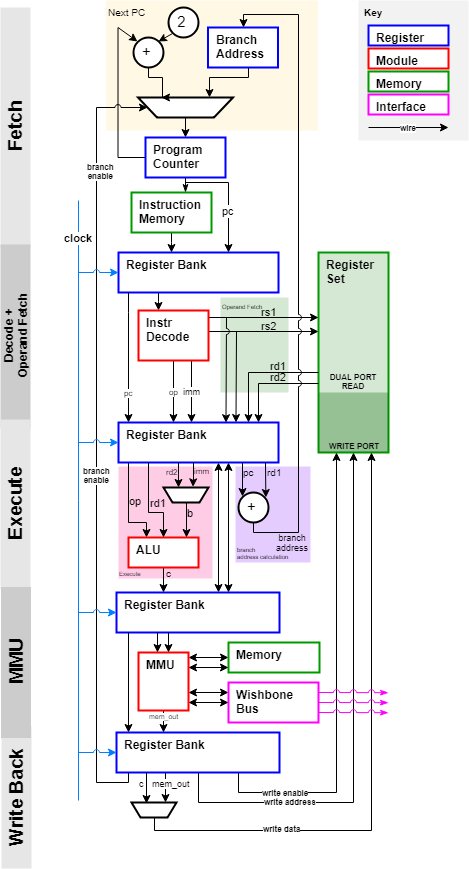
\includegraphics[width=10cm]{../img/risc}
\caption{Vmicro16 RISC 5-stage RTL diagram showing: instruction pipelining (data passed forward through clocked register banks at each stage); branch address calculation; ALU operand calculation (rd2 or imm); and program counter incrementing.}
\label{fig:risc}
\end{figure}

A small reduction in size within the single-core will result in substantial size reductions in 

\subsection{Instruction Set Architecture}
\begin{quotation}
\noindent Core deliverable \ref{cd:isa} details the background for the requirement of a custom instruction set architecture.
\end{quotation}

\noindent
The 16-bit instruction set listing is shown in Figure \ref{fig:isa}.

Most instructions are \textit{destructive}, meaning that source operands also act as the destination, hence effectively \textit{destroying} the original source operand. This design decision reduces the complexity of the ISA as traditional three operand instructions, for example \verb|add r0, r0, r1|, can be encoded using only two operands \verb|add r0, r1|. However, this does increase the complexity of compilers as they may need to make temporary copies of registers as the instructions will \textit{destroy} the original data.

The instruction set is split into 7 categories (highlighted by colours in Figure \ref{fig:isa}): special instructions, such as halting and interrupt returns; memory operations, such as loading and storing; bitwise operations, such as XOR and AND; unsigned arithmetic; signed arithmetic; conditional branches; and atomic load/store instructions.

%The instruction set supports bitwise operations such as OR, XOR, AND, NOT, and left and right shifts. It was decided to provide these functions to enable software to easily create large 16-bit values which is expensive with only an 8-bit immediate.

\subsection{Instruction and Data Memory}
The design uses separate instruction and data memories similar to a Harvard architecture computer. This architecture was chosen due because it is generally easier to implement, however later resulted in design challenges in large multi-core designs. This is discussed later in the report.

\subsection{Memory Management Unit}
It was decided to use a memory management unit (MMU) to make it easier and extensible to communicate with external peripherals or additional registers. This method would transparently use the existing \verb|LW|/\verb|SW| instructions which removes the requirement for a unique instruction for each peripheral. 


\subsection{ALU Design}
The Vmicro16's ALU is an asynchronous module that has 3 inputs: data a; data b; and opcode op; and outputs data c.
The ALU is able to operate on both register data (\verb|rd1| and \verb|rd2|) and immediate values. A switch is used to set the \verb|b| input to either the \verb|rd2| or \verb|imm| value from the previous stage.

\begin{figure}[H]
\centering 
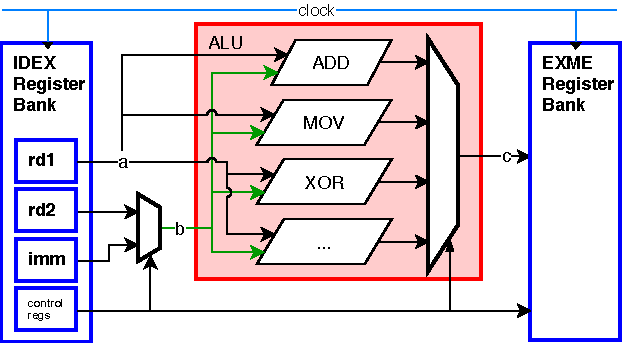
\includegraphics[width=10cm]{../img/alu}
\caption{Vmicro16 ALU diagram showing clocked inputs from the previous IDEX stage being }
\label{fig:alu}
\end{figure}

The ALU also performs comparison (\verb|CMP|) operations in which it returns flags similar to X86's overflow, signed, and zero, flags. The combination of these flags can be used to easily compute relationships between the two input operands. For example, if the zero flag is not equal to the signed flag, then the relationship between inputs $a$ and $b$ is that $a < b$.

\begin{listing}[H]
\centering
\begin{minted}[fontsize=\scriptsize,linenos,baselinestretch=0.5,frame=single,framesep=10pt]{verilog}
module branch (
    input [3:0] flags,
    input [7:0] cond,
    output reg  en
);
    always @(*)
        case (cond)
            `VMICRO16_OP_BR_U:  en = 1;
            `VMICRO16_OP_BR_E:  en = (flags[`VMICRO16_SFLAG_Z] == 1);
            `VMICRO16_OP_BR_NE: en = (flags[`VMICRO16_SFLAG_Z] == 0);
            `VMICRO16_OP_BR_G:  en = (flags[`VMICRO16_SFLAG_Z] == 0) && 
                                     (flags[`VMICRO16_SFLAG_N] == flags[`VMICRO16_SFLAG_V]);
            `VMICRO16_OP_BR_L:  en = (flags[`VMICRO16_SFLAG_Z] != flags[`VMICRO16_SFLAG_N]);
            `VMICRO16_OP_BR_GE: en = (flags[`VMICRO16_SFLAG_Z] == flags[`VMICRO16_SFLAG_N]);
            `VMICRO16_OP_BR_LE: en = (flags[`VMICRO16_SFLAG_Z] == 1) || 
                                     (flags[`VMICRO16_SFLAG_N] != flags[`VMICRO16_SFLAG_V]);
            default:            en = 0;
        endcase
endmodule
\end{minted}
\caption{ALU branch detection using flags: zero (Z), overflow (V), and negative (N).}
\end{listing}


The Verilog implementation of the ALU is shown in \cref{fig:aluv}. The ALU's asynchronous output is clocked with other registers, such as destination register \verb|rs1| and other control signals, in the \verb|EXME| register bank.
\begin{listing}[H]
\centering
\begin{minted}[fontsize=\scriptsize,linenos,baselinestretch=0.5,frame=single,framesep=10pt]{verilog}
always @(*) case (op)
    // branch/nop, output nothing
    `VMICRO16_ALU_BR,
    `VMICRO16_ALU_NOP:          c = {DATA_WIDTH{1'b0}};
    // load/store addresses (use value in rd2)
    `VMICRO16_ALU_LW,
    `VMICRO16_ALU_SW:           c = b;
    // bitwise operations
    `VMICRO16_ALU_BIT_OR:       c = a | b;
    `VMICRO16_ALU_BIT_XOR:      c = a ^ b;
    `VMICRO16_ALU_BIT_AND:      c = a & b;
    `VMICRO16_ALU_BIT_NOT:      c = ~(b);
    `VMICRO16_ALU_BIT_LSHFT:    c = a << b;
    `VMICRO16_ALU_BIT_RSHFT:    c = a >> b;
\end{minted}
\caption{Vmicro16's ALU implementation named vmicro16\_alu. vmicro16.v}
\label{fig:aluv}
\end{listing}




\subsection{Decoder Design}
Instruction decoding occurs in the between the IFID and IDEX stages. 
The decoder extracts register selects and operands from the input instruction. The decoder outputs are asynchronous which allows the register selects to be passed to the register set and register data to be read asynchronously. The register selects and register read data is then clocked into the IDEX register bank.

\begin{listing}[H]
\centering
\begin{minted}[fontsize=\scriptsize,linenos,baselinestretch=0.5,frame=single,framesep=10pt]{verilog}
always @(*) case (opcode)
    `VMICRO16_OP_SPCL: casez(instr[11:0])
        `VMICRO16_OP_SPCL_NOP,
        `VMICRO16_OP_SPCL_HALT,
        `VMICRO16_OP_SPCL_INTR:   alu_op = `VMICRO16_ALU_NOP;
        default:                  alu_op = `VMICRO16_ALU_NOP; endcase
    
    `VMICRO16_OP_LW:              alu_op = `VMICRO16_ALU_LW;
    `VMICRO16_OP_SW:              alu_op = `VMICRO16_ALU_SW;
    `VMICRO16_OP_LWEX:            alu_op = `VMICRO16_ALU_LW;
    `VMICRO16_OP_SWEX:            alu_op = `VMICRO16_ALU_SW;

    `VMICRO16_OP_MOV:             alu_op = `VMICRO16_ALU_MOV;
    `VMICRO16_OP_MOVI:            alu_op = `VMICRO16_ALU_MOVI;
\end{minted}
\caption{Vmicro16's ALU implementation named vmicro16\_alu. vmicro16.v}
\caption{Vmicro16's decoder module code showing nested bit switches to determine the intended opcode. vmicro16.v}
\label{fig:vdecoder}
\end{listing}

In \cref{fig:vdecoder}, it can be seen that the first 8 opcode cases are represented using the same 15-11 bits, however the \verb|VMICRO16_OP_BIT| instructions require another bit range to be compared to determine the output opcode.



\subsection{Pipelining}
In the interim progress update, the processor design featured \textit{instruction pipelining} to meet requirement \ref{ed:ipc}. Instruction pipelining allows instructions executions to be overlapped in the pipeline, resulting in higher throughput (up to one instruction per clock) at the expense of 5-6 clocks of latency and code complexity. As the development of the project shifted from single-core to multi-core, it became obvious that the complexity of the pipelined processor would inhibit the integration of multi-core functionality. It was decided to remove the instruction pipelining functionality and use a simpler state-machine based pipeline that is much simpler to extend and would cause fewer challenges later in the project. 


\section{Verification}
Various verification techniques are employed to ensure correct operation of the processor.

The first technique involves using static assertions to identify incorrect configuration parameters at compile time, such as having zero instruction memory and scratch memory depth. These assertions use the \verb|static_assert| for top level checks and \verb|static_assert_ng| for checks inside \verb|generate| blocks.

The second verification technique is to use assertions in \verb|always| blocks to identify incorrect behavioural states. This is done using the \verb|rassert| (run-time assert) macro.

The third verification technique is to use automatic verifying test benches. These test benches drive components of the processor, such as the ALU and decoder, and check the output against the correct value. This uses the \verb|rassert| macro.

The final method of verification is to verify the complete design via a behavioural test bench. The design is passed a compiled software program with a known expected output, and is ran until the \verb|r_halt| signal is raised. The test bench then checks the value on the \verb|debug0|, \verb|debug1|, and \verb|debug2| signals against the expected value. If this matches, then it is assumed that sub-components of the design also operate correctly. This technique does not monitor the states of sub-components and statistics (such as time taken to execute an instruction), there leaves the possibility that some components could have entered an illegal state.



\subsection{Design Optimisations}
In a design that has many instantiations of the same component, a small resource saving improvement in the component can have a significant overall improvement if it is instantiated many times. Project requirement, \ref{cd:vendor}, requires the design to be compiled for a range of FPGA sizes, and so space saving optimisations are considered. 

\subsubsection{Register Set Size Improvements}
A register set in a CPU is a fast, temporary, and small memory that software instructions directly manipulate to perform computation. In the Vmicro16 instruction set, eight registers named r0 to r7 are available to software. The instruction set allows up to two registers to be references in most instructions, for example the instruction \verb|add r0, r1| tells the processor to perform the following actions:
\begin{enumerate}
\item Fetch r0 and r1 from the register set
\item Add the two values together in the ALU
\item Store the result back the register set in r0
\end{enumerate}
For task 1, it was originally decided to use a dual port register set (meaning that two data reads can be performed in a single clock), however due to the asynchronous design of the register set (for speed) the RTL produced consumed a significant amount of FPGA resources, approximately 256 flip-flops (16 (data width) * 8 (registers) * 2 (ports)). To reduce this, it was decided to split task 1 into two steps over two clock cycles using a single-port register set. This required the processor pipe-line to use another clock cycle resulting in slightly lower performance, however the size improvements will allow for more cores to be instantiated in the design.









